\documentclass{article}
\usepackage{graphicx}
\usepackage{amsmath}
\usepackage{float}
\usepackage{amsfonts}
\usepackage{listings}
\usepackage{xcolor}
\usepackage[utf8]{inputenc}
\usepackage{hyperref}
\usepackage{fancybox}
\usepackage{booktabs}
\usepackage{tikz}
\usepackage[margin=2cm]{geometry}
\usetikzlibrary{shapes, arrows.meta, positioning}
\usepackage[labelfont=bf, font=small]{caption}  % Pour personnaliser le titre de la figure


\lstset{
  language=R,
  basicstyle=\ttfamily\small,
  numbers=left,               % Numérotation des lignes
  numberstyle=\tiny\color{gray}, % Style de la numérotation
  keywordstyle=\color{blue},  % Couleur des mots-clés
  commentstyle=\color{green}, % Couleur des commentaires
  stringstyle=\color{red},    % Couleur des chaînes de caractères
  breaklines=true,            % Coupe les lignes trop longues
  frame=single,               % Encadre le code
}


\title{TP1 TID}
\author{SCAIA Matteo, MARIAC Damien}
\date{\today} 

\begin{document}

\maketitle

\begin{figure}[h] 
    \centering
    
\includegraphics[width=0.5\textwidth]{ssd_logo.png} 
\end{figure}

\begin{figure}[h] 
    \centering
    
\includegraphics[width=0.5\textwidth]{logo_um_2022_rouge_RVB.png} 
\end{figure}

\newpage

\tableofcontents

\newpage
\section{Préambule}
Pour les calculs, nous avons choisit de faire l'exercice 1 (\ref{Exercice1}) en utilisant le logarithme en base 2, et les exercices 2 et 3 (\ref{exercice2} et \ref{exercice3}) en logarithme népérien.\\
Cependant, calculer avec le logarithme népérien ou avec le logarithme en base 2 revient au même. En effet, les deux logarithmes peuvent être reliés par une relation.
 Cela signifie que toute expression impliquant \( \log_2 \) peut être transformée en \( \ln \), et cela ne change pas l'interprétation des résulats. Ils ont seulement un facteur multiplicatif constant les différenciant.

Ces deux logarithmes sont reliés par la formule suivante :

\[
\log_2(x) = \frac{\ln(x)}{\ln(2)}
\]


\section{Exercice 1}
\label{Exercice1}

On considère le tableau ci-dessous, répartissant la population active occupée selon l'âge ($A$), le sexe ($S$) et la
catégorie socioprofessionnelle ($C$) (source: INSEE, enquête emploi 2016).
\begin{figure}[ht]
  \centering
  \setlength{\fboxsep}{0pt}  % Pour que l'image soit bien ajustée dans le cadre
  \setlength{\fboxrule}{1pt}  % Épaisseur du cadre
  \fbox{%
    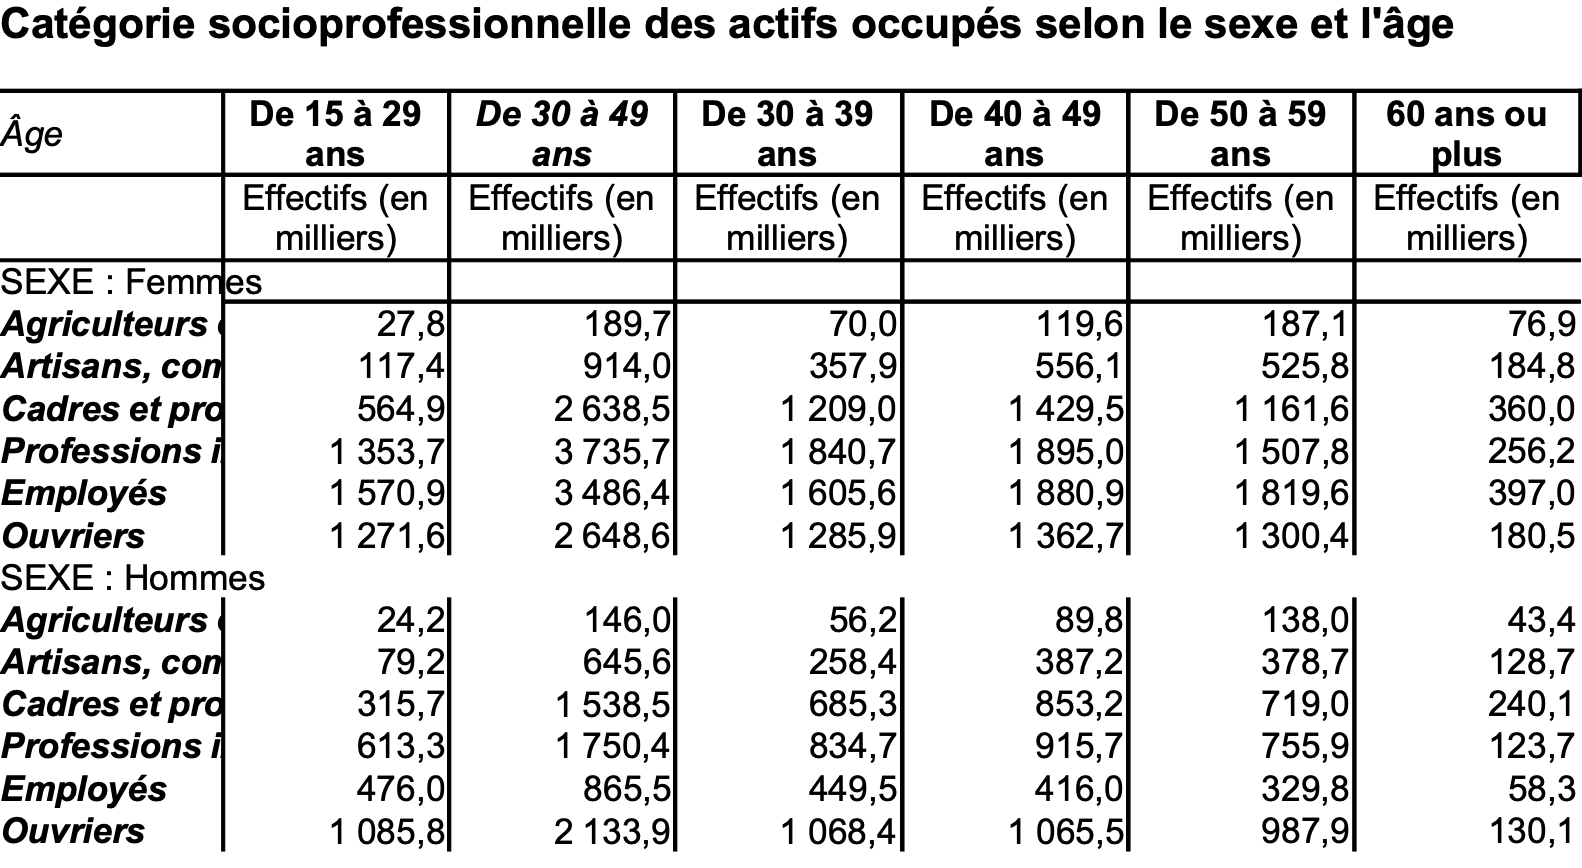
\includegraphics[width=0.7\textwidth]{CE.png}
  }
  \caption{Tableau répartissant la population active occupée selon des catégories }
\end{figure}
\subsection{Modélisation et variable}
\label{1.1}
Tout d'abord de manière intuitive, nous avons envie de modéliser la variable
socioprofessionnelle avec les deux autres. Cependant, nous devons
le montrer de manière formelle. Grâce au code fourni dans la partie \ref{sec : Annexe},
nous calculons l'information mutuelle de chacune des variables.\\\\
Premièrement, nous calculons l'entropie de chacune de ces variables.\\
Pour la variable $A$, nous avons le tableau suivant (en fréquence). 
\begin{table}[ht]
  \centering
  \begin{tabular}{|l|l|l|l|l|l|l|}
    \hline
    & 15-29 ans  & 30-39 ans  & 40-49 ans  & 50-59 ans  & 60+ ans \\ \hline
    Age & 0.1866 & 0.2419 & 0.2730 & 0.2441 & 0.0542 \\ \hline
  \end{tabular}
  \caption{Distribution par âge ($A$)}
\end{table}
\\Nous pouvons calculer l'entropie de $A$.\\
\[
H(A) = -\sum_{n = 1}^{6}p_i\log_2(p_i)=2,1833
\]
De même manière, nous calculons l'entropie de $C$ et $S$.\\
\begin{table}[H]
  \centering
  \begin{tabular}{|l|l|l|}
  \hline
             & Femme  & Homme  \\ \hline
  Proportion & 0,6589 & 0,3411 \\ \hline
  \end{tabular}
  \caption{Distribution par sexe ($S$)}
\end{table}

\begin{table}[H]
  \centering
  \begin{tabular}{|l|l|l|l|l|l|l|}
  \hline
             & Agriculteur & Artisans & Cadres & Profession In & Employes & Ouvrier \\ \hline
  Proportion & 0,0207      & 0,0740   & 0,1875 & 0,2512        & 0,2240   & 0,2423  \\ \hline
  \end{tabular}
  \caption{Distribution par catégorie socioprofessionnelle ($C$)}
  \end{table}


Nous obtenons.
\[
H(S) = 0,9258  \hspace{2 cm} H(C)= 2,3266
\]
A présent, nous devons calculer les valeurs suivantes : $H(A,S)$, $H(A,C)$ et $H(S,C)$.\\
\begin{table}[H]
  \centering
  \begin{tabular}{|l|l|l|l|l|l|}
  \hline
        & 15-29 ans & 30-39 ans & 40-49 ans & 50-59 ans & 60+    \\ \hline
  Femme & 0,1220    & 0,1584    & 0,1803    & 0,1618    & 0,0362 \\ \hline
  Homme & 0,0645    & 0,0834    & 0,0927    & 0,0823    & 0,1802 \\ \hline
  \end{tabular}
  \caption{Distribution jointe sexe ($S$) et âge ($A$)}
  \end{table}

  \begin{table}[H]
    \centering
    \begin{tabular}{|l|l|l|l|l|l|}
    \hline
                   & 15-29 ans & 30-39 ans & 40-49 ans & 50-59 ans & 60+    \\ \hline
    Agriculteur    & 0,0013    & 0,0031    & 0,0052    & 0,0081    & 0,0030 \\ \hline
    Artisans       & 0,0049    & 0,0153    & 0,0234    & 0,0225    & 0,0080 \\ \hline
    Cadres         & 0,0219    & 0,0471    & 0,0568    & 0,0468    & 0,0149 \\ \hline
    Professions In & 0,0489    & 0,0665    & 0,0699    & 0,0563    & 0,0094 \\ \hline
    Employes       & 0,0509    & 0,0511    & 0,0571    & 0,0535    & 0,0113 \\ \hline
    Ouvrier        & 0,0586    & 0,0586    & 0,0604    & 0,0569    & 0,0077 \\ \hline
    \end{tabular}
    \caption{Distribution jointe ($C$) et âge ($A$)}
    
  \end{table}

\begin{table}[H]
  \centering
  \begin{tabular}{|l|l|l|l|l|l|l|}
  \hline
         & Agriculteur & Artisans & Cadres & Profession IN & Employes & Ouvrier \\ \hline
    Femmes & 0.0119      & 0.0433   & 0,1175 & 0.1705        & 0.1810   & 0.1344  \\ \hline
    Homme  & 0.0087      & 0.0307   & 0,0700 & 0.0807        & 0.0430   & 0.1079  \\ \hline
    \end{tabular}
    \caption{Distribution jointe ($C$) et ($S$)}
\end{table}
Nous obtenons les valeurs suivantes.
\[
H(A,S)=3,1092 \hspace{1 cm} H(A,C)= 4,4817 \hspace{1cm} H(C,S)=3,2242
\]
De plus, nous obtenons pour $H(A,S,C)$ la valeur suivante.
\[
  H(A,C,S) = -\sum_{n = 1}^{72}p_i\log_2(p_i)=5,3778
\]
Nous pouvons calculer les informations mutuelles.
\[
I(C,(AS))=H(C)+H(A,S)-H(A,S,C) = 0,0580 \\
\]
\[
I(A,(SC))= 0,029803
\]
\[
I(S,(CA))=0,029813
\]
Cherchons le rapport entre l'information mutuelle et la variable conditionnée le plus élevé.
\[
R_1 = \frac{I(C,(AS))}{H(A,C)}=0,0187
\]
\[
R_2 = \frac{I(A,(SC)))}{H(S,C)}=0,0092
\]
\[
R_3 = \frac{I(S,(CA)))}{H(A,C)}=0,0066
\]
Le rapport $R_1$ est le plus élevé. Donc la variable $C$ modélisé par les deux autres ($A$ et $S$) nous donne le plus d'information.
\subsection{Arbre de segmentation binaire}
Grâce à la partie \ref{1.1}, nous pouvons calculer les informations mutuelles suivantes.
\[
I(A,S) = H(A) + H(S) - H(A,S) = 5,1104*10^{-5}
\]
\[
I(A,C) = 0,02830
\]
\[
I(S,C)= 0,02831
\]
Faisons, la somme de ses informations mutuelles avec chacune des deux autres.
\[
\bar{I_A} = I(A,S) + I(A,C) = 0,02835
\]
\[
\bar{I_S}= 0,02836 
\]
\[
\bar{I_C} = 0,0566
\]
Nous avons donc $\bar{I_C}$ qui est le plus élevé. Ainsi, l'arbre de segmentation commencera avec la variable $C$.






\newpage
\section{Exercice 2}
\label{exercice2}
\subsection{Recodages}

\subsubsection{Recodage en 2 variables}

En agrégeant seulement les classes contigues, nous avons 4 possibilités de regroupement binaire de 
X.
\\
 NB : Dans cette partie, nous effecturons nos calculs avec le log népérien.


\[
Z_1 =\{ \{0 \% \} , \{0 - 0.5 \% ,0.5-1 \% ,1-3 \% ,>3 \% \} \}  
\]
\[
Z_2 =\{ \{0 \% , 0 - 0.5 \%  \} , \{0.5-1 \% ,1-3 \% ,>3 \% \} \}
\]
\[
Z_3 =\{ \{0 \%, 0 - 0.5 \% ,0.5-1 \%  \} , \{1-3 \% ,>3 \% \} \}
\]
\[
Z_4 =\{ \{0 \% , 0 - 0.5 \% ,0.5-1 \% ,1-3 \% \} , \{>3 \% \} \}
\]


L'entropie de chacun de ses recodages se calcule numeriquement et donne :

\[
H(Z_1) = -\left(\frac{29}{72}log_2(\frac{29}{72})+\frac{43}{72}log_2(\frac{43}{72})\right) = 0.973
\]
De la même manière, nous trouvons.
\[
H(Z_2) = 0.954 \hspace{1cm} H(Z_3) = 0.617 \hspace{1cm} H(Z_4) = 0.106
\]
Le meilleur recodage est donc le premiers c'est à dire :
$Z1 =\{ \{0 \% \} , \{0 - 0.5 \% ,0.5-1 \% ,1-3 \% ,>3 \% \} \}$


\subsubsection{Recodage en 3 variables}

En procédant de la meme facon, on considère alors 6 cas :

\[
Z_1 =\{ \{0 \% \} , \{0 - 0.5 \%\} ,\{0.5-1 \% ,1-3 \% ,>3 \% \} \}  
\]
\[
  Z_2 =\{ \{0 \% \} , \{0 - 0.5\%, 0.5-1 \% \} ,\{1-3 \% ,>3 \% \} \}
\]
\[
  Z_3 =\{ \{0 \% \} , \{0 - 0.5\%, 0.5-1 \% ,1-3 \%  \} ,\{>3 \% \} \}
\]
\[
  Z_4 =\{ \{0 \%, 0 - 0.5\%\} , \{ 0.5-1 \% ,1-3 \%  \} ,\{>3 \% \} \}
\]
\[
  Z_5 =\{ \{0 \%, 0 - 0.5\%\} , \{ 0.5-1 \% \} ,\{1-3 \% , >3 \% \} \}
\]
\[
  Z_6 =\{ \{0 \%, 0 - 0.5\%,  0.5-1 \% \} , \{1-3 \%  \} ,\{>3 \% \} \}
\]
\\
L'entropie est calculé numériquement :
\[
H(Z_1) = 1.541 \hspace{0.5cm} H(Z_2) = 1.462 \hspace{0.5cm} H(Z_3) = 1.068 \hspace{0.5cm} H(Z_4) = 1.040 \hspace{0,5cm} H(Z_5) = 1.320 \hspace{0,5 cm} H(Z_6) = 0.684
\]
Nous remarquons que le meilleure recodage en 3 variables est $Z1$.

\subsection{Le meilleur recodage de X pour prédire Y }

Il sagit ici de recoder $X$ en réduisant l'incertitude sur $Y$.
Nous devons donc trouver le $Z_k$ qui maximise l'information mutuelle entre $Z_k$ et Y.
\\
C'est à dire, trouvons le recodage $Z_k$ qui maximise :
\begin{equation}
  I(Z_k; Y) = \sum_{z\in Z_k} \sum_{y \in Y} p(z, y) \log \left( \frac{p(z, y)}{p(z)p(y)} \right)
  \label{eq:infomutu}
\end{equation}

\underline{Détaillons le calcul pour le premier recodage :}

\begin{table}[H]
  \centering
  \begin{tabular}{|l|l|l|}
  \hline
      & 0\%   & $\neq$ 0\% \\ \hline
  OUI & 2/72  & 20/72 \\ \hline
  NON & 27/72 & 23/72 \\ \hline
  \end{tabular}
  \end{table}
Ainsi
\[
p(Z_1 = 0\%) = \frac{29}{72}, \quad p(Z_1 \neq 0\%) = \frac{43}{72}
\]
\[
p(Y = \text{Oui}) = \frac{22}{72}, \quad p(Y = \text{Non}) = \frac{50}{72}
\]
De plus

\[
p(Z_1 = 0\%, Y = \text{Oui}) = \frac{2}{72}, \quad p(Z_1 = 0\%, Y = \text{Non}) = \frac{27}{72}
\]
\[
p(Z_1 \neq 0\%, Y = \text{Oui}) = \frac{20}{72}, \quad p(Z_1 \neq 0\%, Y = \text{Non}) = \frac{23}{72}
\]
Nous pouvons calculer l'information mutuelle $I(Z1,Y)$, en utilisant la formule \ref{eq:infomutu}.
\[
I(Z_1; Y) = p(Z_1 = 0\%, Y = \text{Oui}) \log_2 \left(\frac{p(Z_1 = 0\%, Y = \text{Oui})}{p(Z_1 = 0\%) p(Y = \text{Oui})}\right) + \ldots
\]
\[
+ p(Z_1 = 0\%, Y = \text{Non}) \log_2 \left(\frac{p(Z_1 = 0\%, Y = \text{Non})}{p(Z_1 = 0\%) p(Y = \text{Non})}\right) + \ldots
\]
\[
+ p(Z_1 \neq 0\%, Y = \text{Oui}) \log_2 \left(\frac{p(Z_1 \neq 0\%, Y = \text{Oui})}{p(Z_1 \neq 0\%) p(Y = \text{Oui})}\right) + \ldots
\]
\[
+ p(Z_1 \neq 0\%, Y = \text{Non}) \log_2 \left(\frac{p(Z_1 \neq 0\%, Y = \text{Non})}{p(Z_1 \neq 0\%) p(Y = \text{Non})}\right)
\]
Nous trouvons alors:
\[
  I(Z_1; Y)= 0.176
\]
Faisons le même cheminement mais avec les autres variables. Nous obtenons alors les informations mutuelles suivante.
\[
I(Z_1,Y) = 0.176
\]

\[
I(Z_2,Y) = 0.091
\]

\[
I(Z_3,Y) = 0.033
\]

\[
I(Z_4,Y) = 0.024
\]
On observe que l'information mutuelle la plus élevé est $I(Z_1,Y)$. Donc le recodage avec la variable $Z_1$ est le meilleur permettant de prédire $Y$.


\newpage
\section{Exercice 3}
\label{exercice3}
\subsection{Description}

On considère le tableau recensant des espèces de champignons suivant 4 variables qualitatifs. 

\begin{table}[h]
  \centering
  \caption{Caractéristiques des espèces de champignons}
  \begin{tabular}{@{}ccccc@{}}
  \toprule
  Espèce & Comestible & Chapeau & Tige & Couleur \\ \midrule
  a      & o          & a       & e    & b       \\
  b      & o          & a       & e    & j       \\
  c      & o          & a       & e    & b       \\
  d      & o          & pl      & f    & j       \\
  e      & o          & pl      & f    & b       \\
  f      & n          & po      & f    & r       \\
  g      & n          & po      & f    & j       \\
  h      & n          & po      & e    & r       \\
  i      & n          & a       & f    & j       \\
  j      & n          & pl      & f    & j       \\ \bottomrule
  \end{tabular}
  
  \label{tab:champignons}
  \end{table}

  On cherche à faire un arbre de discrimination qui permet de prédire la comestibilité à partir des autres caractéristiques, tout en étant le plus court possible.
  \\
  \\
  Pour ce faire, on calcul les informations mutuelles de $X_1$ avec chaque autre variable.
  En effet, nous allons chercher la variables qui informe le plus sur la commestibilité. Nous effecturons nos calculs avec le logarithme népérien.

Nous posons pour la suite
\[
X_1 = \{Comestible\} \hspace{1cm} X_2 = \{Chapeau\} \hspace{1cm} X_3 = \{Tige\} \hspace{1cm} X_4 = \{Couleur\}
\]

\subsection{Calculs}

\subsubsection{Premiere étape}
On calcul l'information mutuelle avec la formule suivante, $I(X_1,X_2) = H(X_1) + H(X_2) - H(X_1,X_2)$.

\begin{table}[H]
  \centering
    \caption{Croissement entre comestibilité $(X_1)$ et forme du chapeau $(X_2)$}
    \begin{tabular}{|l|l|l|l|}
    \hline
    X1\textbackslash{}X2 & Po & a & Pl \\ \hline
    O                    & 0  & 3 & 2  \\ \hline
    N                    & 3  & 1 & 1  \\ \hline
    \end{tabular}
\end{table}
Nous trouvons grâce à ce tableau, $I(X_1,X_2)$=$H(X_1)+H(X_2)-H(X_1,X_2)$=0.277.
\\\\
Pour les variables suivantes, nous avons ces tableaux.

\begin{table}[H]
  \centering
    \caption{Croisement entre comestibilité $(X_1)$ et la tige $(X_3)$}
    \begin{tabular}{|l|c|c|}
    \hline
    $X_1 \backslash X_3$ & e & f \\ \hline
    O                    & 3  & 2  \\ \hline
    N                    & 1  & 4  \\ \hline
    \end{tabular}
\end{table}

\begin{table}[H]
  \centering
    \caption{Croisement entre comestibilité $(X_1)$ et la couleur $(X_4)$}
    \begin{tabular}{|l|l|l|l|}
      \hline
      $X_1\backslash X_2$ & b & j & r \\ \hline
      O                    & 3  & 2 & 0  \\ \hline
      N                    & 0  & 3 & 2  \\ \hline
      \end{tabular}
\end{table}

De la même manière, nous pouvons calculer l'information mutuelle et nous trouvons :




\[
  I(X_1,X_3)=0.106 \hspace{1cm} I(X_1,X_4)=0.357
\]




Nous pouvons conclure a cette étape que la variable qui apporte le plus d'information sur la comestibilité du champignon est la couleur du champignon. En effet, l'information mutuelle $I(X_1,X_4)$ est la plus élevé.
\\
De plus, on se rend compte dans le tableau \ref{tab:champignons} que les champignons brun sont commestibles alors que les rouges ne le sont pas.
\\
Traitons le cas des champignons jaune.
    
\subsubsection{Deuxieme étape : champignons jaune}
En considérant que les champignons jaune, on calcul les informations mutuelles suivant les autres variables ($X_2$ et $X_3$). Nous obtenons les tableaux suivant.

\begin{table}[H]
  \caption{Tableau de $X_1$,$X_2$ avec champignon jaune}
  \centering
  \begin{tabular}{|l|l|l|l|}
  \hline
  $X_1\backslash X_2$ & a & pl & po \\ \hline
  O                    & 1 & 1  & 0  \\ \hline
  N                    & 1 & 1  & 1  \\ \hline
  \end{tabular}
  \end{table}

\begin{table}[H]
  \centering
  \caption{Tableau de $X_1$,$X_3$ avec champignon jaune}
  \begin{tabular}{|l|l|l|}
  \hline
  $X_1\backslash X_3$ & e & f \\ \hline
  O                    & 1 & 1 \\ \hline
  N                    & 0 & 2 \\ \hline
  \end{tabular}
  \end{table}
Nous calculons les informations mutuelles et nous obtenons les résultats suivant.
\[
  I(X_1,X_2)=0.118 \hspace{1cm} I(X_1,X_3)=0.223.
\]

On considère alors la variable $X_3$, celle qui correspond à la tige du champignon. Si le champignon est jaune et épais, alors il est commestible. Sinon il faut distinguer entre le champignon d (commestible) et les champignons g,i,j.

\newpage
\subsection{Arbre de discrimination}

Avec toutes les informations mutuelles calculé, on obtient alors l'arbre suivant :



\begin{figure}[htbp]
  \centering
  \resizebox{\textwidth}{!}{
  \begin{tikzpicture}[
    every node/.style={draw, rectangle, rounded corners, align=center, minimum size=10mm, font=\scriptsize},
    level 1/.style={sibling distance=100mm},
    level 2/.style={sibling distance=70mm},
    level 3/.style={sibling distance=35mm},
    level 4/.style={sibling distance=40mm},
    edge from parent/.style={draw, -{Latex[length=5mm]}, thick},
    level distance=35mm
  ]
  
  \node {Couleur}
    child {node {rouge}
        child {node {f,h} edge from parent node[right] {Non comestible}}
    }
    child {node {tige}
        child {node {Epaisse}
            child {node {b} edge from parent node[right] {Comestible}}
        }
        child {node {fine}
            child {node {type chapeau}
                child {node {pointu}
                    child {node {non commestible}}
                }
                child {node {arrondi}
                    child {node {non commestible}}
                }
                child {node {plat}
                    child {node {j}
                        child {node {non commestible}}
                    }
                    child {node {d}
                        child {node {commestible}}
                    }
                }
            }
        }
    }
    child {node {brun}
        child {node {a,c,e} edge from parent node[right] {Comestible}}
    };
  \end{tikzpicture}
  }
\caption{Arbre de discrimination pour la comestibilité d'un champignon}
\end{figure}
\end{document}



\newpage
\section{ANNEXE}
\label{sec : Annexe}
\end{document}
